\documentclass{article}

\usepackage[L7x,T1]{fontenc}
\usepackage[utf8]{inputenc}
\usepackage{csquotes}
\usepackage[english]{babel}
\usepackage[maxbibnames=99,style=authoryear]{biblatex}
\addbibresource{bib.bib}
\usepackage{hyperref}
\usepackage{caption}
\usepackage{subcaption}
\usepackage{gensymb}
\usepackage{varwidth}
\usepackage{tikz}
\usetikzlibrary{er,positioning}

\title{
    Cartografic Generalization of Lines \\
    (example of rivers) \\ \vspace{4mm}
}

\author{Motiejus Jakštys}

\date{\today}

\begin{document}
\maketitle

\newpage

\section{Abstract}
\label{sec:abstract}

Current open-source line generalization solutions have their roots in
mathematics and geometry, thus emit poor cartographic output. Therefore, if one
is using open-source technology to create a large-scale map, downscaled lines
(e.g. rivers) will not be professionally scale-adjusted. This paper explores
line generalization algorithms and suggests one for an avid GIS developer to
implement. Once it is usable from within open-source GIS software (e.g. QGIS or
PostGIS), rivers on these large-scale maps will look professionally downscaled.

\section{Introduction}
\label{sec:introduction}

Cartographic generalization is one of the key processes of creating large-scale
maps: how can one approximate object features, without losing its main
cartographic properties? The problem is universally challenging across many
geographical entities (\cite{muller1991generalization},
\cite{mcmaster1992generalization}). This paper focuses on line generalization,
using natural rivers as examples.

Line generalization algorithms are well studied, tested and implemented, but
they expose deficiencies in large-scale reduction (\cite{monmonier1986toward},
\cite{mcmaster1993spatial}). Most of these techniques are based on mathematical
shape representation, rather than cartographic characteristics of the line.

In this paper we explore algorithms which are derived from cartographic
knowledge and processes, so their output is as similar as an experienced
cartographer would create, thus most correct and visually appealing.

We will be using a small part of Žeimena:

\begin{figure}
    \centering
    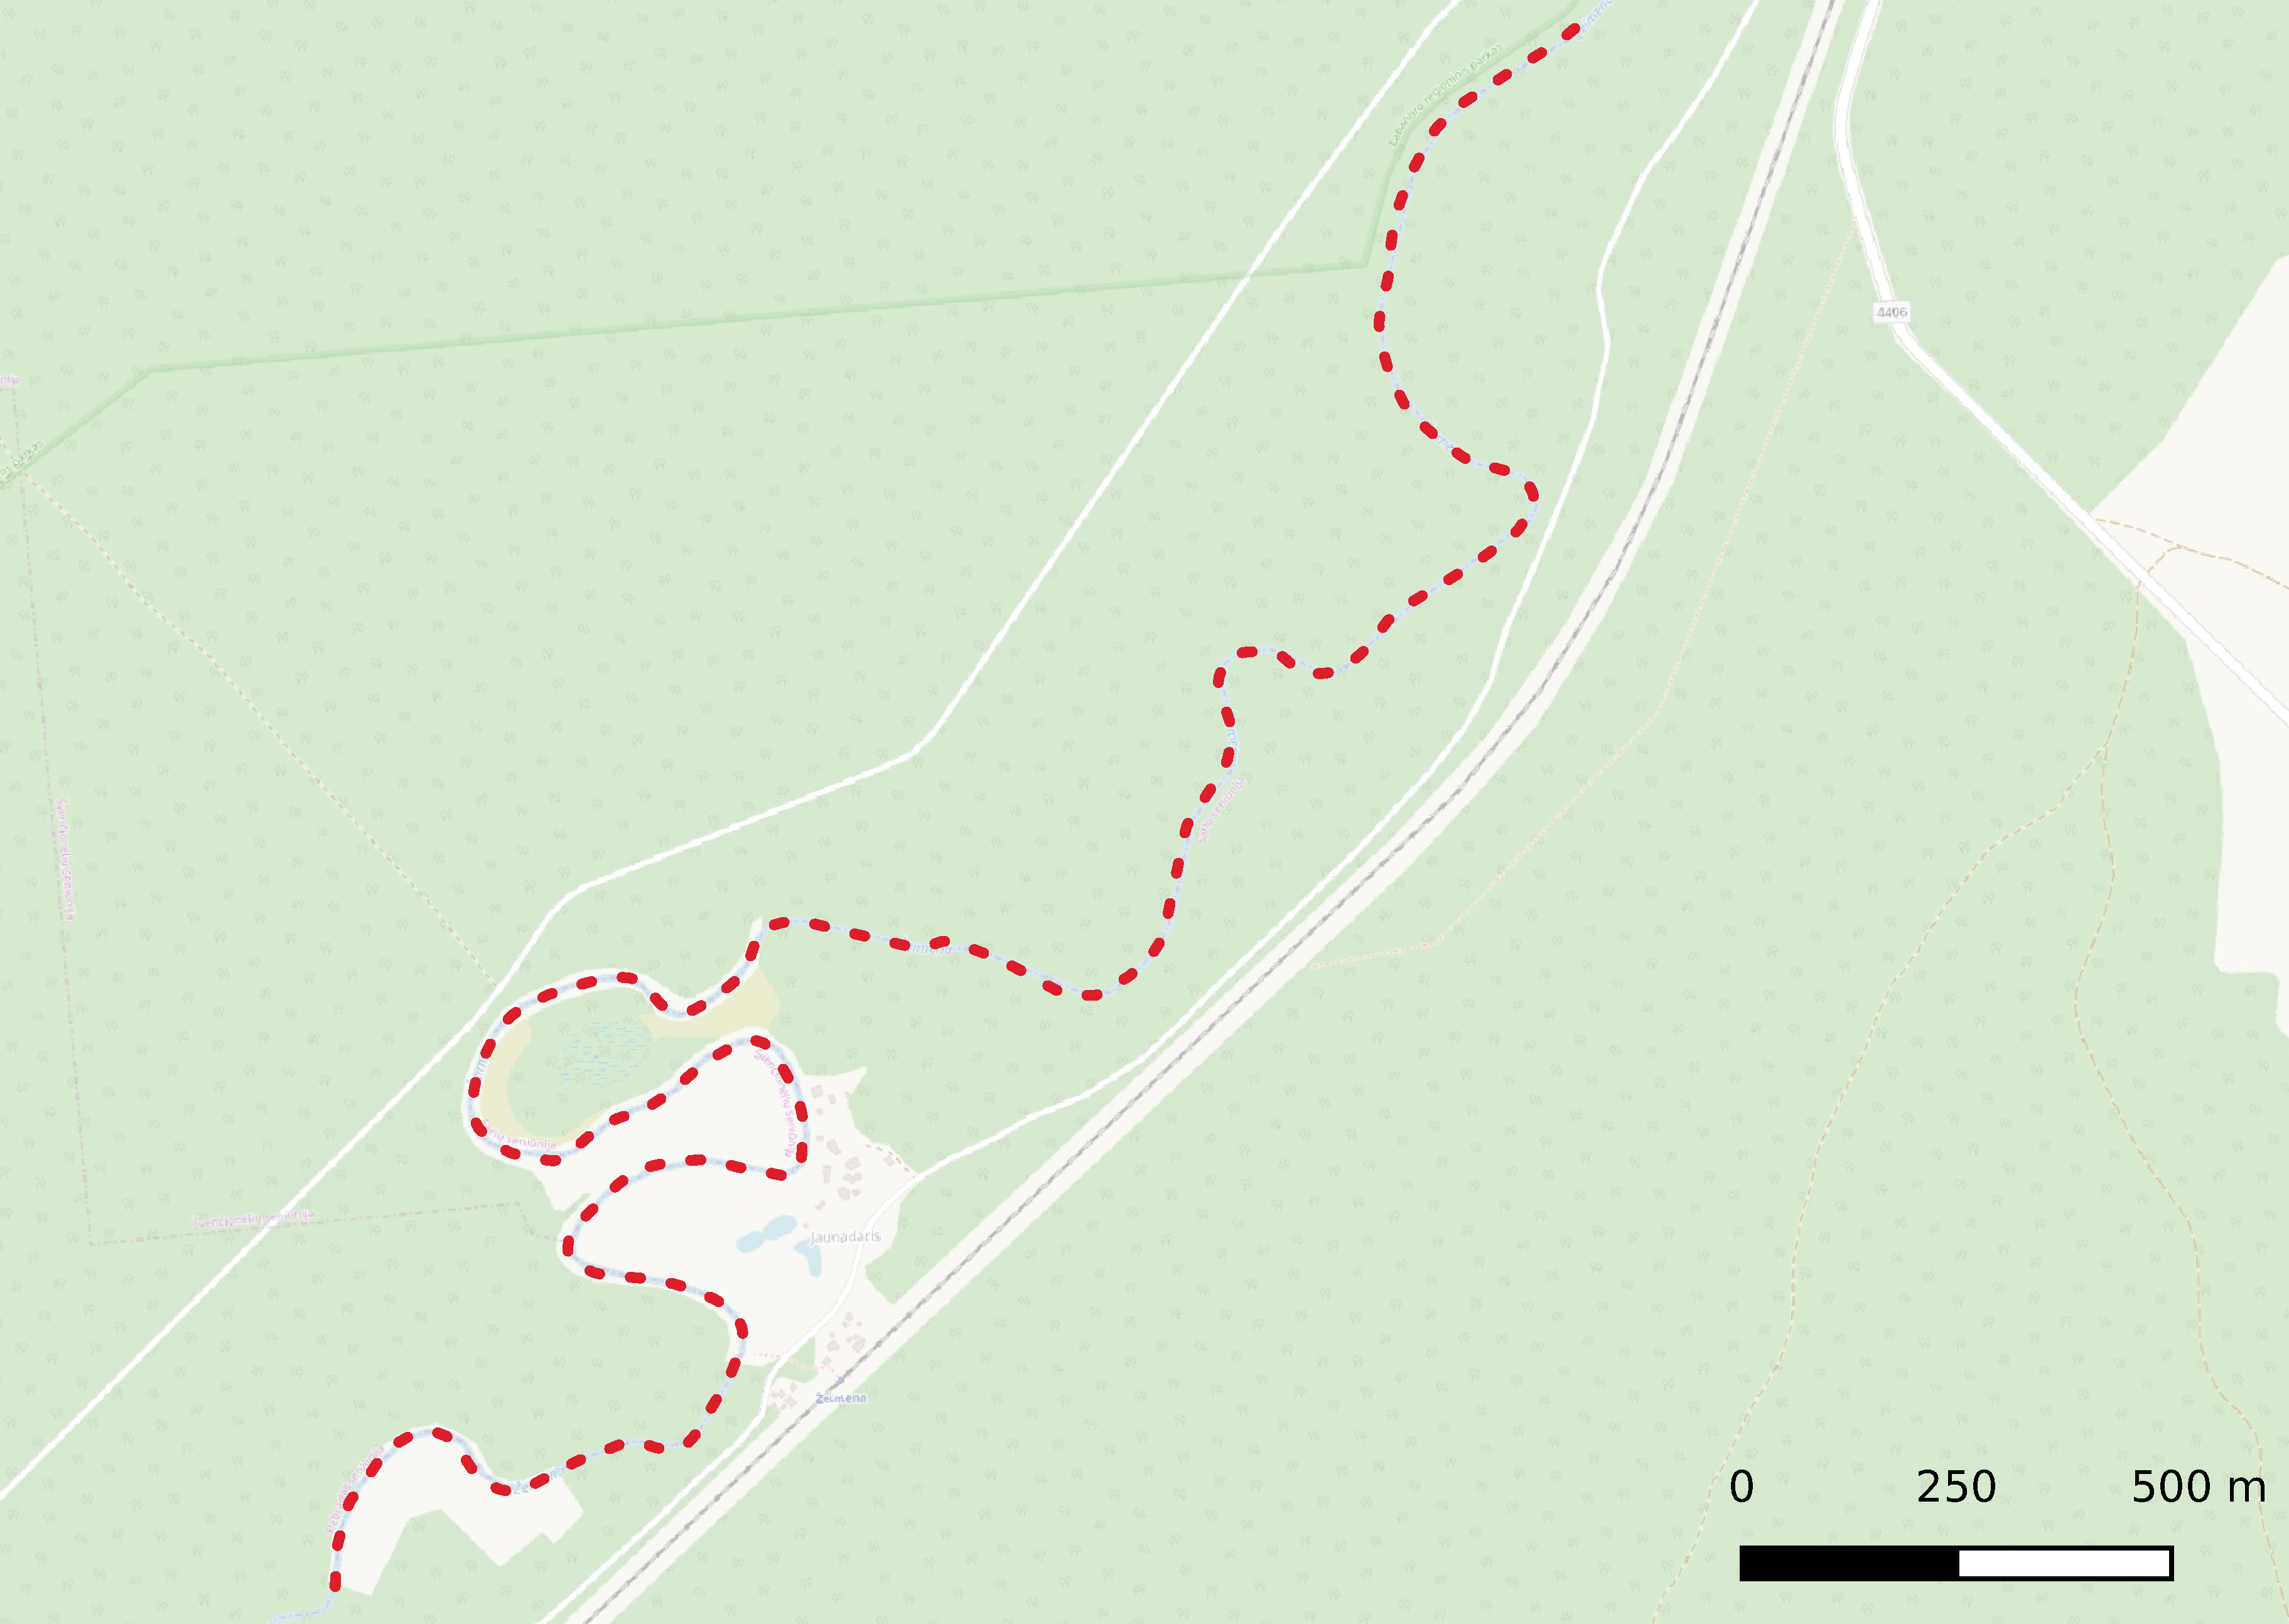
\includegraphics[width=\textwidth]{zeimena}
    \caption{Žeimena near Jaunadaris}
\end{figure}

\section{Mathematical and geometrical algorithms}

To understand why geometrical algorithms are not entirely suitable for 
downscaling, let's pick some visual examples.

\subsection{Douglas \& Peucker}

\cite{douglas1973algorithms} is one of the most well-known line simplification algorithm.


\section{Algorithms based on cartographical knowledge}

\cite{jiang2003line}, \cite{dyken2009simultaneous},
\cite{mustafa2006dynamic}, \cite{nollenburg2008morphing}

\section{My Idea}
\label{sec:my_idea}

\section{Related Work}
\label{sec:related_work}

\cite{stanislawski2012automated} studied different types of metric assessments,
such as Hausdorff distance, segment length, vector shift, surface displacement,
and tortuosity for the generalization of linear geographic elements. Their
research can provide references to the appropriate settings of the line
generalization parameters for the maps at various scales.


\section{Conclusions and Further Work}
\label{sec:conclusions_and_further_work}

\printbibliography

\end{document}
